\documentclass[xcolor=svgnames,final,smaller,a4]{beamer}
% rubber: module beamer
% rubber: module pdftex
% rubber: module graphics
% rubber: set program pdflatex-escape
%% should have a script named pdflatex-escape e.g. in ~/bin/ like
%%  #! /bin/sh -x
%%  exec pdflatex -shell-escape $*
%
%
%
\usepackage[english]{babel}
\usepackage[T1]{fontenc}
\usepackage[utf8]{inputenc}
\usepackage{multicol}
\usepackage{minted}
\usepackage{pstricks}
\usepackage{relsize}
\usepackage{times}
\usepackage{alltt}
\usepackage{url}
\usepackage{hyperref}
\usepackage{verbatim}
\usepackage{textcomp} % for \texttrademark
\usepackage{wasysym} % wasysym for \smiley & \frownie{} 
\usepackage{xspace}

% wolverine beamer/themes/color/beamercolorthemewolverine.sty
\definecolor{darkblue}{rgb}{0,0,0.8}

\setbeamercolor{alerted text}{fg=darkblue!80!yellow}
\setbeamercolor*{palette primary}{fg=darkblue!60!black,bg=yellow!85!orange}
\setbeamercolor*{palette secondary}{fg=darkblue!70!black,bg=yellow!60!orange}
\setbeamercolor*{palette tertiary}{bg=darkblue!80!black,fg=yellow!50!orange}
\setbeamercolor*{palette quaternary}{fg=darkblue,bg=yellow!20!orange}

\setbeamercolor*{sidebar}{fg=darkblue,bg=orange!75!white}

\setbeamercolor*{palette sidebar primary}{fg=darkblue!10!black}
\setbeamercolor*{palette sidebar secondary}{fg=white}
\setbeamercolor*{palette sidebar tertiary}{fg=darkblue!50!black}
\setbeamercolor*{palette sidebar quaternary}{fg=yellow!10!orange}

\setbeamercolor*{titlelike}{parent=palette primary}
\setbeamercolor{frametitle}{bg=yellow!90!orange}
\setbeamercolor{frametitle right}{bg=yellow!60!orange}

\setbeamercolor*{separation line}{fg=orange:20!nay}
\setbeamercolor*{fine separation line}{}

% AnnArbor beamer/themes/theme/beamerthemeAnnArbor.sty 
\useinnertheme[shadow=true]{rounded}

% beamer/themes/outer/beamerouterthemeinfolines.sty
\setbeamercolor*{author in head/foot}{parent=palette tertiary}
\setbeamercolor*{title in head/foot}{parent=palette secondary}
\setbeamercolor*{date in head/foot}{parent=palette primary}

\setbeamercolor*{section in head/foot}{parent=palette tertiary}
\setbeamercolor*{subsection in head/foot}{parent=palette primary}

\defbeamertemplate*{footline}{infolines theme}
{
  \leavevmode%
  \hbox{%
  \begin{beamercolorbox}[wd=.22\paperwidth,ht=2.25ex,dp=1ex,center]{author in head/foot}%
    \usebeamerfont{author in head/foot}\insertshortauthor
  \end{beamercolorbox}%
  \begin{beamercolorbox}[wd=.33\paperwidth,ht=2.25ex,dp=1ex,center]{title in head/foot}%
    \usebeamerfont{title in head/foot}\insertshorttitle
  \end{beamercolorbox}%
  \begin{beamercolorbox}[wd=.45\paperwidth,ht=2.25ex,dp=1ex,right]{date in head/foot}%
    \usebeamerfont{date in head/foot}\insertshortdate{}\hspace*{2em}
   {\ifthenelse{\boolean{XTRASLIDE}}{\textcolor{red}{$\spadesuit$}}{$\star$}}
    {\scriptsize\insertframenumber{}} / {\inserttotalframenumber}\hspace*{2ex} 
  \end{beamercolorbox}}%
  \vskip0pt%
}

\defbeamertemplate*{headline}{infolines theme}
{
  \leavevmode%
  \hbox{%
  \begin{beamercolorbox}[wd=.5\paperwidth,ht=2.25ex,dp=1ex,right]{section in head/foot}%
    \usebeamerfont{section in head/foot}\insertsectionhead\hspace*{2ex}
  \end{beamercolorbox}%
  \begin{beamercolorbox}[wd=.5\paperwidth,ht=2.25ex,dp=1ex,left]{subsection in head/foot}%
    \usebeamerfont{subsection in head/foot}\hspace*{2ex}\insertsubsectionhead
  \end{beamercolorbox}}%
  \vskip0pt%
}

\setbeamersize{text margin left=1em,text margin right=1em}


\setbeamerfont{block title}{size={}}
\setbeamercolor{titlelike}{parent=structure,bg=yellow!85!orange}

\renewcommand{\theFancyVerbLine}{\sffamily
\textcolor{FireBrick}{\scriptsize
\oldstylenums{\arabic{FancyVerbLine}}}}

\newcommand{\petitun}[1]{{\relsize{-1}{#1}}}
\newcommand{\prodname}[1]{\textcolor{DarkGreen}{\textsf{\relsize{-0.5}#1}}}
\newcommand{\melt}{\prodname{Melt}\xspace}
\newcommand{\gcc}{\prodname{Gcc}\xspace}
\newcommand{\mailto}[1]{{\href{mailto:#1}{\small{{\texttt{#1}}}}}}
\newcommand{\petitdemi}[1]{{\relsize{-0.5}{#1}}}
\newcommand{\mongra}[1]{\textcolor{red}{\textbf{#1}}}
\newcommand{\monimp}[1]{\textcolor{Purple}{\textbf{#1}}}
\newcommand{\monbleu}[1]{\textcolor{DarkBlue}{\textbf{#1}}}
\newcommand{\monbric}[1]{\textcolor{FireBrick}{\textbf{#1}}}
\newcommand{\monvert}[1]{\textcolor{DarkGreen}{{#1}}}
\newcommand{\moncomm}[1]{\monvert{\textbf{\emph{#1}}}}

%%% flag for extra slides with xslide environment
\newboolean{XTRASLIDE}
\setboolean{XTRASLIDE}{false}

\newenvironment{mslide}%
{\setbeamercolor{normal text}{bg=yellow!10}%
%\setbeamertemplate{footline}{\insertframenumber/\inserttotalframenumber} 
\setbeamercolor{titlelike}{parent=structure}
\setbeamercovered{transparent}%
\begin{frame}[containsverbatim]}%
{\end{frame}}

\newenvironment{xslide}%
{\setbeamercolor{normal text}{bg=red!20}%
%\setbeamertemplate{footline}{\textcolor{red}{$\oplus$}~\insertframenumber/\inserttotalframenumber}% 
\setbeamercolor{titlelike}{parent=structure}%
\setbeamercovered{transparent}%
\setboolean{XTRASLIDE}{true}%
\begin{frame}[containsverbatim]}%
{\end{frame}}%

\newenvironment{myalltt}%
{\begin{relsize}{-1.5}\begin{alltt}}%
{\end{alltt}\end{relsize}}

\AtBeginSection[]{\begin{mslide}\begin{relsize}{-0.5}\tableofcontents[currentsection]
    \end{relsize}
\end{mslide}}


\begin{document}
\title[metaprogramming for the Web?]{metaprogramming for the Web? \\
  \vspace{0.2cm}
  \small{(newbie intro to \href{http://www.open-source-innovation-spring.org/techniques-de-programmation-web-letat-de-lart-date-conf/}{OSIS2016 \monbric{``state of the art web technologies''} workshop})}}
\author[Basile Starynkevitch]{Basile \textsc{Starynkevitch} \\
\href{http://gcc-melt.org/}{\textcolor{Navy}{\bf\texttt{\large gcc-melt.org}}} and \href{http://starynkevitch.net/Basile/}{\textcolor{Navy}{\bf\texttt{starynkevitch.net/Basile/}}} \\
\href{mailto:basile@starynkevitch.net}{\textcolor{Blue}{\texttt{basile@starynkevitch.net}}} 
  or
  \href{mailto:basile.starynkevitch@cea.fr}{\textcolor{Blue}{\texttt{basile.starynkevitch@cea.fr}}}}

\institute[CEA, LIST]
{\begin{tabular}[c]{ccc}

\includegraphics[height=1.1cm]{CEA-LIST-logo-cote} %
& \hspace{0.3cm}\raisebox{0.22cm}{
\includegraphics[width=2.5cm]{Systematic-GT-LogicielLibre}} %
&  \hspace{0.3cm}\raisebox{0.22cm}{
\includegraphics[width=2.5cm]{logoIRILL}} \\
  \end{tabular}\\
  {\relsize{-0.5}{CEA, LIST (Software Reliability Lab.), Palaiseau, France}}\\
  {\relsize{-2}{[within Université Paris Saclay]}}
}

\date[June 28\textsuperscript{th}, 2016 ~ (OSIS2016)]%
{\small June 28\textsuperscript{th}, 2016, \\
  \href{http://www.open-source-innovation-spring.org}{\textcolor{DarkGreen}{\emph{Open Source Innovation Spring}}}, Jussieu, Paris, France}

\begin{frame}
  \maketitle
  
\end{frame}



 \begin{mslide}
   \frametitle{Overview}
   \tableofcontents

   \begin{center}
     \begin{relsize}{-2}
       
       Slides available at
       \href{http://starynkevitch.net/Basile/starynkevitch-osis2016.pdf}{\textcolor{Navy}{\bf\texttt{starynkevitch.net/Basile/starynkevitch-osis2016.pdf}}}
       \\ under \,
       \raisebox{-0.2em}{
\includegraphics[width=0.10\textwidth]{cc-by-sa}} \hspace{3em}
                {\relsize{-1}{(Creative Commons Attribution Share
                    Alike 4.0 International license)}}

  \LaTeX {/} Beamer source code on \href{https://github.com/bstarynk/osis2016webtech/}{\textcolor{Brown}{\bf\texttt{github.com/bstarynk/osis2016webtech/}}}
     \end{relsize}


     \medskip
     
 {All \mongra{opinions are mine only}} 
   \end{center}
 \end{mslide}
 
%\begin{xslide}
%\begin{block}{\textcolor{Red}{\textbf{\Large Caveat}}}
%{\Large All \textbf{opinions are mine only}} 
%\end{block}
%
%\begin{itemize}
%\item I (Basile) don't speak for my employer, CEA (or my institute LIST)
%  \item I don't speak for Systematic or IRILL
%\item I don't speak for the GCC community
%\item I don't speak for anyone else
%\item My opinions may be highly controversial
%\item My opinions may change
%\item \monimp{I am a web \emph{newbie}}
%  \item I use Linux (only), even for browsing the Web
%\end{itemize}
%
%\end{xslide}



 %%%%%%%%%%%%%%%%%%%%%%%%%%%%%%%%%%%%%%%%%%%%%%%%%%%%%%%%%%%%%%%%
 \section{Introduction}

 \begin{mslide}
   \frametitle{Introduction ~ {\relsize{-1}{(audience)}}}
   Expected \mongra{audience} {\relsize{-1}{(OSIS2016)}} :
   \begin{itemize}
   \item \monimp{developers} curious of Web technologies
   \item \mongra{\emph{web developers}} curious on non-mainstream Web technologies
   \item \monimp{free-software friendly} and knowledgable
   \end{itemize}
 \end{mslide}
 
 \begin{mslide}
   \frametitle{Why am \emph{I} \petitun{(Basile)} interested by web technologies?}
   \begin{itemize}
   \item I am a compiler \& static source code analysis guy (\href{http://gcc-melt.org/}{\prodname{\bf \texttt{gcc-melt.org}}}), \petitun{very far from the Web!}
   \item Web technologies are about \monimp{half} of IT economy
   \item static source analysis tools \mongra{need} \monimp{powerful user interfaces}\\
     \petitun{(because they compute a \emph{lot} of things)}
   \item GUI toolkits (e.g. Qt) are becoming \emph{out of fashion}
     \item many companies dislike installing software on their own
       developer's laptops, prefering Web applications \petitun{(running elsewhere)}
     \item I feel the need for a persistent tool with a web interface \petitun{(``MELT monitor'', for a \emph{small} team working on the same software)}
     \item \monimp{I am still learning}, and a Web newbie!
       \item I am \mongra{old} enough \petitun{(born in 1959, grandfather)} to not have
         learned anything about the Web
         \item I have lots of questions! (perhaps better answered offline)
   \end{itemize}
 \end{mslide}

 \begin{mslide}
   \frametitle{History and evolution of the \emph{World Wide Web}}
   
 Cf \href{http://www.evolutionoftheweb.com}{\monbleu{\texttt{evolutionoftheweb.com}}} \& wikipage \href{https://en.wikipedia.org/wiki/History_of_the_World_Wide_Web}{\monbric{History of the World Wide Web}}
   \petitun{\begin{itemize}
     
   \item \emph{Tim Berner Lee}'s pionnering work at CERN: 1980 -
     \monimp{1990}: web for helping scientists to work together (distributed hypertext)
     
     \item \mongra{HTTP} \petitun{(HyperText Transfer Protocol)}, a textual client-server protocol \petitun{(HTTP 0.9 in 1990, HTTP 1.1 in 1997-\monimp{1999} \href{https://tools.ietf.org/html/rfc2616}{\emph{RFC2616}}, HTTP 2 in \monimp{2015} for 8\% of websites today)}.

     \item \mongra{HTML} \petitun{(HyperText Markup Language, inspired by SGML)}, evolved as HTML4 (1997) \& HTML5 (2007) with Canvas, Video, etc...
     \item \mongra{URL}s \petitun{(Uniform Resource Locator, RFC1738 in 1994)}
     \item \mongra{CSS} \petitun{(Cascading Style Sheet, 1996; CSS3 modules, 2011; CSS4 WIP)}

     \item \mongra{JavaScript} \petitun{(developed in \emph{10 days \monimp{!}} in may 1995, by B.Eich at Netscape)}; now standardized as \monimp{ECMAScript 7} \petitun{(June 2016)} \& \mongra{DOM}  \petitun{(document object model, DOM1 by W3C 1998, DOM4 by WHATWG, 2015)}

     \item \mongra{AJAX} \petitun{(asynchronous JavaScript \& XML, Feb. 2005; precursor ActiveX at MicroSoft -1999- \& \texttt{XMLHttpRequest} in  Gecko -2000-)}

       \item \mongra{WebAssembly} \petitun{(2016, inspired by \texttt{PNaCl}, Google, 2011)}
   \end{itemize}}

   \monimp{Web technologies evolved \emph{organically}}, no ``grand design'' \petitun{(economical \& social pressure)}, so \mongra{complex} \& \monimp{layered}
 \end{mslide}

 \begin{mslide}
   \frametitle{evolution of the number of websites}
   
   \begin{center}
     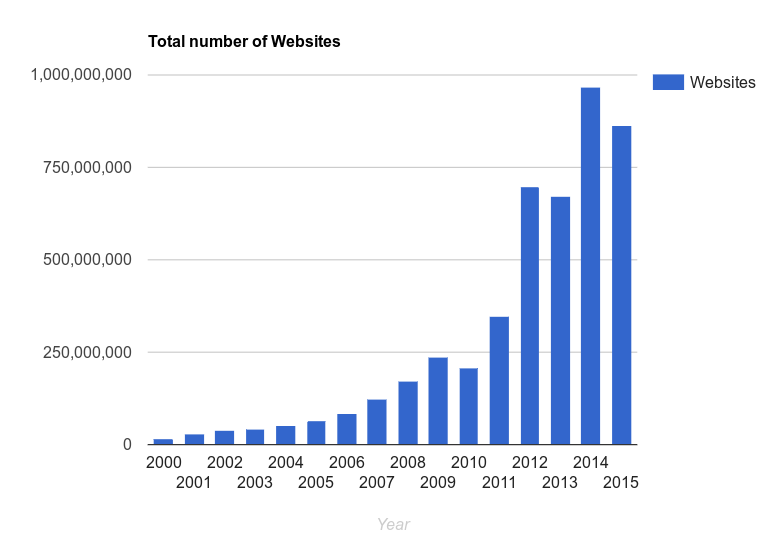
\includegraphics[width=0.75\textwidth]{Total-number-of-Websites}
     
   \smallskip

   \small{From {\href{http://www.internetlivestats.com/total-number-of-websites/#trend}{\textcolor{Brown}{\petitun{\bf\texttt{http://www.internetlivestats.com/total-number-of-websites/}}}}}}
   \end{center}
   
 \end{mslide}
   
 \begin{mslide}
   \frametitle{growth of web page size \& number of objects}

   \begin{center}
     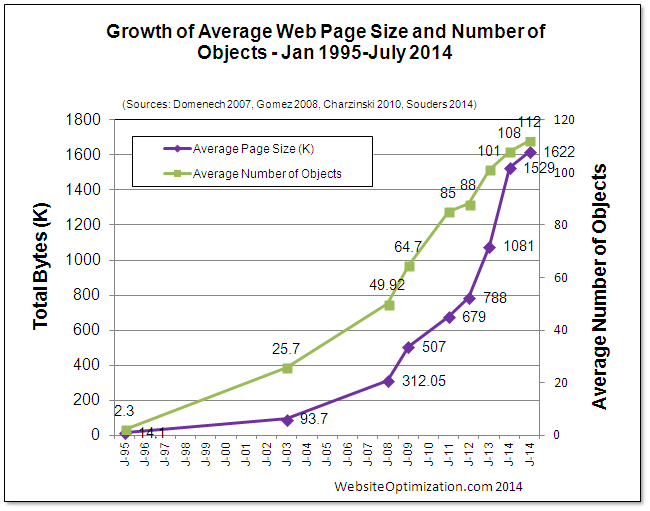
\includegraphics[width=0.77\textwidth]{growth-page-size}
   \end{center}
 \end{mslide}

 \begin{mslide}
   \frametitle{Web technologies ``outside'' of, or ``close'' to, the Web}
   \begin{itemize}
     \item \mongra{web indexing}
   \item \monimp{hidden} web (see \href{https://en.wikipedia.org/wiki/Robots_exclusion_standard}{\monvert{\bf\texttt{robots.txt}} ``standard''})
   \item \monimp{embedded} web servers: user interfaces of printers, routers, \ldots ; free software HTTP server libraries \petitun{(\href{https://www.coralbits.com/libonion/}{\monbleu{libonion}}, \href{http://www.webtoolkit.eu/wt}{\monbleu{Wt}}, \href{http://projects.camlcity.org/projects/ocamlnet.html}{\monbleu{ocamlnet}}, etc \ldots)}
   \item \monimp{mobile} web
   \item \href{https://en.wikipedia.org/wiki/Web_service}{\monimp{web services}} - using \href{https://en.wikipedia.org/wiki/SOAP}{\monbric{SOAP} \petitun{(Simple Object Access Protocol, W3C, 2000)}}, often \href{https://en.wikipedia.org/wiki/Representational_state_transfer}{\monbric{REST}-ful} \petitun{(Representational state transfer, R.Fielding 2000)}
   \item \href{http://json.org/}{\mongra{JSON}} (a notation, 2001, used for Ajax) \&  \href{http://jsonrpc.org/}{\monimp{JSON-RPC}}
   \item embeddable HTTP clients (\href{http://curl.haxx.se/libcurl/}{\monvert{\bf\texttt{libcurl}}}...) \& browsers (\href{http://www.qtweb.net/}{\monbleu{\texttt{QtWeb}}}, \href{https://webkit.org/}{\monbleu{\texttt{WebKit}}}...)
   \item \href{http://fastcgi.com/}{\monvert{\bf\texttt{FastCGI}}} to connect a software to a running web server
     \item Proxies \& \href{https://en.wikipedia.org/wiki/Internet_Content_Adaptation_Protocol}{\monimp{ICAP}} \petitun{(Internet Content Adaptation Protocol, 1999)}
   \end{itemize}
 \end{mslide}



 %%%%%%%%%%%%%%%%%%%%%%%%%%%%%%%%%%%%%%%%%%%%%%%%%%%%%%%%%%%%%%%%
 \section{[Meta-] programming for the web}
 
 \begin{mslide}
   \frametitle{Generating HTML}

   \begin{itemize}
   \item \mongra{PHP} \petitun{(R.Lerdorf, 1994; PHP7: 2015, faster!)}: dynamically typed interpreter
   \item and many \monimp{other tools}, sometimes generating HTML in batch
     \begin{itemize}
     \item \href{http://hevea.inria.fr/}{\monvert{\bf\texttt{HeVeA}}}, a \LaTeX $~\rightarrow~$ HTML5 converter
     \item zillions of HTML \monimp{generators}
     \item many HTML \monimp{editors}
     \end{itemize}
     \item several libraries, e.g. \href{http://freemarker.org/}{\monbleu{FreeMarker}} (for Java) etc, \& ``template engines''
   \item some interesting but dead languages: \href{https://sourceforge.net/projects/kaya/}{\monbric{Kaya}}, etc \ldots
   \end{itemize}
   \bigskip
   But what about \monimp{JavaScript}?
 \end{mslide}

 \begin{mslide}
   \frametitle{Issues in JavaScript}

   Today (2016) JavaScript is \petitun{[nearly]} \monimp{the \emph{only} way to code for the browser}.
   
   \petitun{\small(but JavaScript was designed \& implemented in only \emph{ten days}!)}

   \medskip
   
   JavaScript is:

   \begin{itemize}
   \item \monimp{hard} to learn \petitun{(books of 800-1000 pages)} with \monimp{weird syntax \& \emph{semantics}} \footnote{~ \petitun{\monbleu{\url{https://wiki.haskell.org/The_JavaScript_Problem}}}}
   \item difficult prototype based object model ; dynamically typed
   \item \monimp{difficult} to implement efficiently
     \item have a big and \monimp{complex \emph{specification}} \petitun{($\approx 566$ pages, \href{http://www.ecma-international.org/ecma-262/7.0/}{\prodname{EcmaScript$_{v7}$}}, 2016)}
   \item here to stay, \mongra{won't disappear} soon!
   \item \mongra{many criticisms} available on the web (and security\footnote{~ \petitun{\monbleu{\url{http://www.ssi.gouv.fr/uploads/IMG/pdf/NP_Securite_Web_NoteTech.pdf}}}, in French.\\} issues)
   \item many \monimp{frameworks} and \monimp{toolkits} (\href{http://jquery.org/}{\prodname{JQuery}}, \ldots)
   \item better \monimp{generated} than handwritten
   \end{itemize}
 \end{mslide}

 \begin{mslide}
   \frametitle{headache with browser $\leftrightarrow$ server executions}
   
Some \mongra{dynamic behavior inside the web browser} is required, notably in \href{https://en.wikipedia.org/wiki/Single-page_application}{\monimp{single-page web applications}}
   \begin{itemize}
   \item server initialize the web page at first HTTP requests
   \item actual content is dynamic \petitun{(JavaScript code in
     browser handling events and modifying the DOM)}
   \item most of the page content gets filled after \monimp{asynchronous} \prodname{AJAX} requests
   \item
     \href{https://en.wikipedia.org/wiki/WebSocket}{\prodname{WebSocket}}-s
     enable \monimp{asynchrony}: the server would send some messages
     (often JSON) to the browser
   \end{itemize}
   \bigskip
   \monimp{execution \mongra{oscillates} between web server and browser}, giving motion sickness:
   \begin{itemize}
   \item C.Queinnec's talk {\large \mongra{Continuations \& the web}}
   \item G.Potdevin's talk {\large \mongra{Control inversion in web development}}
   \end{itemize}
   \medskip
   
   \monimp{$\Rightarrow$} better \monimp{generate code mix} in server and browser thru \mongra{meta-programs}
 \end{mslide}

 
 \begin{mslide}
   \frametitle{meta-programming the web}

   Many \petitun{(non-mainstream)} tools and languages are producing code both in browser and in server:

   \begin{itemize}
     
   \item \href{http://opalang.org/}{\prodname{Opa}} - a typesafe language for full-stack application (generates: server program for \prodname{Node.js} + browser program in \prodname{JavaScript} + database for \prodname{MongoDb})
     
   \item \href{http://haxe.org/}{\prodname{Haxe}} - an open source toolkit and language

     \item M.Serrano's talk on \\ {\large \mongra{Mixing computation in web
         server and in browser}}
       (\href{http://hop.inria.fr}{\prodname{HOP}})


     \item V.Balat's talk on \\
       {\large \mongra{Developing multi-platform web \& mobile applications}}
       (\href{http://ocsigen.org/}{\prodname{Ocsigen}})
       
   \end{itemize}
   
 \end{mslide}


 %%%%%%%%%%%%%%%%%%%%%%%%%%%%%%%%%%%%%%%%%%%%%%%%%%%%%%%%%%%%%%%%
 \section{A few newbie technical questions}


 \begin{mslide}
   \frametitle{is \monbric{\texttt{contenteditable}} useful?}

   \petitun{(in the context of some ``syntax directed editor'' or ``AST wiki'')}

   \bigskip

   
   See \href{https://medium.engineering/why-contenteditable-is-terrible-122d8a40e480}
        {\monbleu{why is \monbric{\texttt{contenteditable}} terrible?}} \petitun{(N.Santos, Medium, 2014)}

        \medskip
        
   \hrule
   
   \bigskip
        \begin{itemize}
        \item how to disambiguate cursor position \\
          \petitun{\bf\texttt{\mongra{\large$\mid$}<em><a href='http://example.com/'>some link</a> here</em>}} \\
          vs \\
          \petitun{\bf\texttt{<em>\mongra{\large$\mid$}<a href='http://example.com/'>some link</a> here</em>}}


        \item \monimp{exhaustive} list of user actions and events modifying the editable element? Relation to \monbric{\texttt{execCommand}}?

        \item W3C Editor's draft {\relsize{-2}{\monbleu{\url{https://w3c.github.io/editing/contentEditable.html}}}} - dream or \petitun{\monbric{\texttt{contenteditable='events'}}} soon implemented?

        \item \monbric{\texttt{beforeinput}} \& \monbric{\texttt{input}} events?
          
        \end{itemize}
        
 \end{mslide}

 \begin{mslide}
   \frametitle{dealing with the clipboard (copy \& paste)}

   Traditional (e.g X11
   \href{https://specifications.freedesktop.org/wm-spec/wm-spec-latest.html}{\monbric{EWMH}}
   - \petitun{Extended Window Manager Hints}) clipboard involves a
   \emph{negotiation} on the exchange format or MIME type
   \petitun{(plain text, rich text, image, HTML, \ldots)}. So copying \& pasting
   some web page fragment to LibreOffice preserves italics, but
   copying the same to a terminal only sends text.

   \begin{block}{exchanging structured data}

     Could two similar web applications exchange e.g. JSON data during copy \& paste ? How?
   \end{block}
   
 \end{mslide}
 
 \begin{mslide}
   \frametitle{Security issues?}

   \begin{block}{need of better static analysis tools?}

     Is there a need (\& a ``market'') for open source static analysis tools for Web programming languages?
     
   \end{block}

   \bigskip

   \petitun{(perhaps security is not relevant enough on the web \ldots)}
 \end{mslide}
 
\end{document}

%%%%%%%%%%%%%%%%%%%%%%%%%%%%%%%%%%%%%%%%%%%%%%%%%%%%%%%%%%%%%%%%
%% Local Variables: ;;
%% compile-command: "rubber -d starynkevitch-osis2016" ;;
%% End: ;;
%%%%%%%%%%%%%%%%%%%%%%%%%%%%%%%%%%%%%%%%%%%%%%%%%%%%%%%%%%%%%%%%
